%\part*{Lezione 12/04/2021}
\chapter{$R$-MATRIX}\label{sec-R-mat}
In questo capitolo viene presentato il metodo della $R$-Matrix sia \textit{calculable} che \textit{phenomenological} con alcuni esempi di applicazione. Il capitolo copre le lezioni 12/04/2021, 14/04/2021, 

\paragraph{Introduzione} Finora abbiamo visto che i metodi \textit{ab-initio}\index{metodo ab-initio@metodo \textit{ab-initio}} permettono di calcolare la sezione d'urto partendo da una buona base teorica senza la necessità di \vir{aggiustare} i risultati con osservazioni per ottenere le corrette relazioni, tuttavia dipendono fortemente dal metodo di calcolo delle funzioni d'onda, il quale diviene sempre più complesso al crescere di $A$. In questo capitolo tratteremo quindi le caratteristiche principali di un metodo alternativo a quello \textit{ab-initio} detto metodo della $R$-MATRIX (RM)\index{metodo Rmatrix@metodo $R$-MATRIX} seguendo l'articolo di Descouvemont \& Baye\footnote{\label{0412_art} Descouvemont, P. \& Baye, D., Rep. Prog. Phys., 2010, vol.3, \texttt{DOI:} \doi{10.1088/0034-4885/73/3/036301}, \texttt{arXiv:} \url{https://arxiv.org/abs/1001.0678}.\articolo{Descouvemont \& Baye}}.\\ 
Esistono due principali versioni:
\begin{enumerate}
	\item \textit{Phenomenological}\index{metodo Rmatrix@metodo $R$-MATRIX!Phenomenological}
	\item \textit{Calculable}\index{metodo Rmatrix@metodo $R$-MATRIX!Calculable}
\end{enumerate}
Il primo a essere stato sviluppato è stato 1., ma dal punto di vista didattico è più chiaro il 2., per cui partiremo da questo.

\section{Calculable RM}\index{metodo Rmatrix@metodo $R$-MATRIX!Calculable}\label{sec-RM-C}
Studiamo lo scattering $A_1 + A_2$ all'energia $E$. Trascurando per semplicità lo \textit{spin}, sviluppiamo in armoniche sferiche la soluzione dell'equazione di \Sch{}\footnote{L'Hamiltoniana è simmetrica sotto rotazioni, traslazioni e riflessioni.} $(T+V)\psi = E\psi$:
$$\psi = \sum_\ell \frac{u_\ell (r)}{r}\mathcal{Y}_{\ell m}(\hat{r})$$
% $$\PPq{\underbrace{-\frac{\hbar^2}{2\mu}\Bigl (\frac{d^2}{dr^2} -\frac{\ell(\ell+1)}{r^2}}_{T_\ell}- \underbrace{V(r)}_{V_N + V_{coul}}\Bigr )-E} u_\ell(r) =0$$
Raccogliendo i vari termini in $H_\ell\equiv T_\ell + V_C + V_N$ si ha:
\begin{equation}\label{0412_sch}
	(H_\ell - E) u_\ell (r) =0
\end{equation}
\begin{figure}[h]
	\centering
	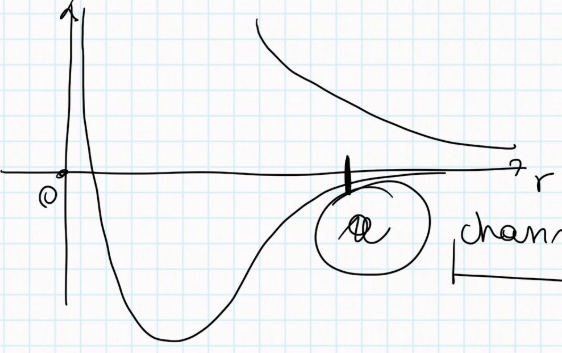
\includegraphics[scale=0.5]{Immagini/0412_potschem.png}
	\caption{Schema del potenziale usato: $V_N$ per $r<a$ e $V_C$ per $r>a$.}
	\label{0412_pot}
\end{figure}
\newline
\noindent Per quanto riguarda il potenziale una schematizzazione come quella in Figura \ref{0329_schema} è troppo semplice, prenderemo invece un potenziale simile a quello in Figura \ref{0412_pot} con un certo raggio $a$ detto \textit{channel radius}\index{channel radius@\textit{channel radius}} che separa la regione interna dove il contributo maggiore è dato da $V_N$ da quella esterna in cui domina $V_C$.\\ 
Partiamo dalle soluzioni per $r>a$:
$u_\ell^{ext} (r) \propto \cos{\delta_\ell} F_\ell (\eta, kr) + \sin{\delta_\ell}G_\ell (\eta,kr)$
dove $F$ e $G$ sono le funzioni di Coulomb\index{funzioni di Coulomb} e $\eta$ è il coefficiente di Coulomb\index{coefficiente di Coulomb}. Definiamo:
$$ I_\ell (kr) \equiv G_\ell (\eta,kr) - i\, F_\ell(\eta,kr) $$
$$ O_\ell (kr) \equiv G_\ell (\eta,kr) + i\, F_\ell(\eta,kr) $$
\begin{equation}\label{0412_uext}
u_\ell^{ext} (r) = C_\ell \ppc{I_\ell(kr) - \underbrace{U_\ell}_{\exp{(2i\delta_\ell)}}O_\ell(kr)}
\end{equation}
Dal momento che si trascurano gli \textit{spin} non si hanno canali accoppiati.\\ 
Per $r<a$ espandiamo in funzioni $\varphi_j$ note e nulle per $r\to0$: %%! Che funzioni sono?????
\begin{equation}\label{0412_uint}
u_\ell^{int} (r) = \sum_{j=1}^N c_j \,\varphi_j(r)
\end{equation}
Sono quindi da determinare solo le costanti $C_\ell$ e $c_j$ attraverso le condizioni di continuità:
\begin{equation}\label{0412_cont}
\Bigl \{
\begin{array}{l}
u_\ell^{int}(a) = u_\ell^{ext}(a)\\ 
u_\ell'^{int}(a) = u_\ell'^{ext}(a)	
\end{array}
\end{equation}
Abbiamo però una difficoltà: $H_\ell$ non è hermitiano in $[0,a]$, quindi non è simmetrico:
\begin{displaymath}
	\begin{aligned}
	\int_0^a dr\, \varphi_i \frac{d^2}{dr^2} \varphi_j &\not = \int_0^a dr\, \varphi_j \frac{d^2}{dr^2} \varphi_j \\ 
	\varphi_i (a) \frac{d}{dr}\varphi_j(a)-\int_0^a dr\,\frac{d}{dr}\varphi_i \frac{d}{dr}\varphi_j &\not = \varphi_j (a) \frac{d}{dr}\varphi_i (a) - \int_0^a dr\,\frac{d}{dr}\varphi_j \frac{d}{dr}\varphi_i  \\
	\varphi_i (a) \frac{d}{dr}\varphi_j(a) &\not = \varphi_j (a) \frac{d}{dr}\varphi_i (a) 
	\end{aligned}
\end{displaymath}
Per questa ragione \vir{\textit{hermitizzeremo}} l'operatore tramite quello che viene definito operatore di Bloch\index{operatore di Bloch}:
\begin{equation}\label{0412_bloch}
\mathscr{L}(B) = \frac{\hbar^2}{2\mu}\delta(r-a) \ppc{\frac{d}{dr}-\frac{B}{r}}
\end{equation}
il risultato non dovrà ovviamente dipendere dal parametro $B$ scelto. Avremo quindi una nuova hamiltoniana $H_\ell \to H_\ell + \mathscr{L}(B)$ hermitiana e l'equazione di \Sch{} diverrà l'equazione di Bloch-\Sch{}\footnote{Per passare da una all'altra è sufficiente sommare da ambo i lati $\mathscr{L}(B)\, u_\ell^{int}$.}:
\begin{equation}\label{0412_blocsch}
\Bigl ( H_\ell + \mathscr{L}(B)-E \Bigr ) u_\ell^{int} = \frac{\hbar^2}{2\mu} \delta(r-a) \Bigl ( \frac{d}{dr} - \frac{B}{r} \Bigr ) u_\ell^{int} = \mathscr{L}(B)\, u_\ell^{ext} 
\end{equation}
dove l'ultima uguaglianza deriva dalla condizione di continuità in $r=a$ (imposto dalla $\delta$) in equazione \eqref{0412_cont}. Definiamo allora la matrice $R$ \index{R-Matrix@$R$-Matrix} come:
\begin{equation}\label{0412_Rl}
u_\ell (a) \equiv R_\ell (E,B) [a \, u_\ell ' (a) - B u_\ell (a)]
\end{equation}
$$\frac{1}{R_\ell (E,B)} \equiv a \frac{u'}{u}\Bigl |_{r=a} - B$$
Sostituendo l'espressione di $u^{int}$ definita in equazione \eqref{0412_uint} nell'equazione \eqref{0412_blocsch}:
\begin{displaymath}
	\begin{aligned}
	\sum_j (H_\ell + \mathscr{L}(B)-E) \, c_j \varphi_j(r) &= \mathscr{L}(B) u_\ell^{ext} \\
	\sum_{j} \, \underbrace{\int_0^a dr\, \varphi_i (r) (H_\ell + \mathscr{L}(B)-E) \, \varphi_j(r) }_{C_{ij}(E,B)}\, c_j &= \int_0^a dr \, \varphi_i(r) \frac{\hbar}{2\mu} \delta(r-a) \ppc{u_\ell'^{ext}(r) - B\frac{u^{ext}_\ell (r)}{r}} \\ 
	\sum_j C_{ij}(E,B)\, c_j &= \frac{\hbar^2}{2\mu a} \varphi_i(a) \ppc{a u_\ell '^{ext} (a) - B u_\ell^{ext} (a)} 
	\end{aligned}
\end{displaymath}
dove $C_{ij}(E,B)$ sono elementi di una matrice simmetrica facilmente calcolabili dal momento che le $\varphi$ sono note; pure le $u_\ell '^{ext} (a)$ e $u_\ell^{ext} (a)$ sono note per cui dall'ultima equazione si possono calcolare i coefficienti $c_j$ e riscrivere in maniera più compatta:
\begin{equation}\label{0412_eq9}
\sum_j C_{ij}(E,B) \, c_j = \frac{\hbar^2}{2\mu a} \varphi_i(a)	\, \frac{u_\ell^{ext}}{R_\ell(E,B)}
\end{equation}
Possiamo da questa ricavare un'espressione per $R_\ell$ partendo dalla \eqref{0412_uint}:
$$u_\ell^{int}(a) = \sum_j \varphi_j(a) \: \sum_i  \pp{[}{C(E,B)}{]}_{ij}^{-1} \varphi_i(a) \frac{\hbar^2}{2\mu a} \frac{u_\ell^{ext}(a)}{R_\ell(E,B)}$$
\begin{equation}\label{0412_uint2}
	u_\ell^{int}(a) = \frac{\hbar^2}{2\mu a} \frac{u_\ell^{ext}(a)}{R_\ell(E,B)} \:  \sum_{i,j=1}^N \varphi_j(a) \pp{[}{C(E,B)}{]}_{ij}^{-1} \varphi_i (a)
\end{equation}
Usando la continuità:
\begin{equation}\label{0412_Rl2}
R_\ell(E,B) = \frac{\hbar^2}{2\mu a} \sum_{i,j=1}^N \varphi_i(a)\, \pp{[}{C(E,B)}{]}_{ij}^{-1}\, \varphi_j(a) 
\end{equation}
Ricordiamo che il potenziale che viene usato non è quello di un singolo nucleone, ma quello di uno o due cluster e questo lo distingue da un metodo \textit{ab-initio}\index{metodo ab-initio@metodo \textit{ab-initio}}.

\subsection{Proprietà della RM}
Supponiamo che $N$ sia finito e le $\varphi$ siano ortonormali. Per $E=0$, poiché la matrice $[C]_{ij}$ è diagonalizzabile, avremo autovettori $\bar{v}_{n\ell}$ (che prendiamo ortonormali) e autovalori $E_{n\ell}$ per cui $C(0,B)\bar{v}_{n\ell} = E_{n\ell} \bar{v}_{n\ell}$. Possiamo allora fare una decomposizione spettrale del tipo $C_{ij}(0,B) = \sum_n E_{n\ell} \bar{v}_{n\ell,i} \bar{v}^T_{n\ell,j}$, da cui sfruttando l'ortonormalità delle $\varphi$ si ha:

$$ C_{ij}(E,B) = \oss{\varphi_i}{H_\ell + \mathscr{L}(B) - E}{\varphi_j} = C_{ij}(0,B) - E\: \delta_{ij} = \sum_{n=1}^N (E_{n\ell} - E)\, \bar{v}_{n\ell,i}\bar{v}^T_{n\ell,j}$$
Sostituendo nella \eqref{0412_Rl2}:
$$R_\ell (E,B) = \frac{\hbar^2}{2\mu a} \sum_{i,j =1}^N \varphi_i(r) \: \sum_{n=1}^{N} \frac{\bar{v}_{n\ell,i}\bar{v}^T_{n\ell,j}}{E_{n\ell}-E} \: \varphi_j$$ 

\noindent Per rendere l'espressione più compatta\footnote{Questa è l'espressione che solitamente si trova per $R$, dove si evidenzia il fatto che è una funzione \textit{meromorfa}\index{funzione meromorfa}, cioè olomorfa ovunque eccetto in una serie di punti isolati.} definiamo la \textit{reduced width}\index{reduced width@\textit{reduced width}} $\gamma_{n\ell} = \sqrt{\hbar^2/2\mu a} \: \phi_{n\ell}(a)$ dove abbiamo definito\footnote{Se $N$ è finito, allora $\phi_{n\ell}$ sono l'approssimazione variazionale delle autofunzioni dell'operatore $H+\mathscr{L}$ in $a$ e l'espressione per $R$ diviene un'approssimazione.} le funzioni d'onda $\phi_{n\ell}(r) = \sum_i \bar{v}_{n\ell,i}\varphi_i(r)$:
\begin{equation}\label{0412_Rl3}
R_\ell (E,B) = \sum_{n=1}^N \frac{\gamma_{n\ell}^2}{E_{n\ell}-E}	
\end{equation}

\subsection{Sfasamento e RM}
Per trovare una relazione tra la matrice di sfasamento $U_\ell$ in \eqref{0412_uext} e la matrice $R_\ell$ eguagliamo\footnote{Adottiamo la notazione per cui l'apice $'$ indica la derivata rispetto all'argomento della funzione:%
\begin{displaymath}%
\begin{array}{l}
	f'(r) = df/dr \\
	g'(kr) = dg/d(kr)
\end{array}
\end{displaymath}%
} l'espressione \eqref{0412_uext} con la definizione \eqref{0412_Rl} per $u^{ext}_\ell (a)$:
$$ C_\ell \PPq{I_\ell(ka) - U_\ell \, O_\ell(ka)} = u_\ell^{ext} = R_\ell(E,B) \,[a \, u_\ell^{ext\,\prime}  (a) - B u_\ell^{ext}] $$
$$U_\ell = \frac{I_\ell(ka)}{O_\ell(ka)} \frac{1+B\, R_\ell -R_\ell \, \overbrace{ka \, I_\ell ' (ka)/I_\ell (ka)}^{L_\ell^*}}{1+B\, R_\ell - R_\ell \, \underbrace{ka \,  O_\ell ' (ka)/O_\ell (ka)}_{L_\ell}}$$
dove abbiamo definito le quantità $L_\ell$ e $L_\ell^*$. Ricordando l'espressione per $I_\ell$ e $O_\ell$ possiamo definire un'angolo di sfasamento $\Phi_\ell$ che caratterizza il contributo coulombiano secondo:
$$\frac{I_\ell (ka)}{O_\ell (ka)} = \frac{\ppc{1-i \, F_\ell/G_\ell}^2}{1 + (F_\ell/G_\ell)^2} = \PPc{\frac{1-i\, F_\ell/G_\ell}{\sqrt{1 + (F_\ell/G_\ell)^2}}}^2 \equiv e^{i2\Phi_\ell}$$
$$\tan{\Phi_\ell} = - F_\ell / G_\ell\Bigl |_{ka}$$
Per cui otteniamo un'espressione di $U_\ell$ che è indipendente da $B$\footnote{Non è evidente, ma è possibile dimostrarlo; non siamo interessati al conto, la dimostrazione è riportata in Complementi \secrif{compl-CRM-dim}.} (come atteso): 
$$U_\ell = e^{2i\Phi_\ell} \, \frac{1-L_\ell^* \, R_\ell (E)}{1-L_\ell  \, R_\ell (E)}$$
Questa relazione può essere usata anche per determinare l'accuratezza del metodo numerico. 
%? (valutando appunto la dipendenza dal parametro $B$)
%! Questo sopra l'ho detto io e secondo me ci sta 
\\
Possiamo ancora però lavorare con tale espressione per raggiungere una forma più compatta e che evidenzi maggiormente la relazione con lo sfasamento $\delta_\ell$. Scriviamo $L_\ell = S_\ell + i \, P_\ell$, dove abbiamo definito $S_\ell$ \textit{shift factor}\index{shift factor@\textit{shift factor}} e $P_\ell$ \textit{penetration factor}\index{penetration factor@\textit{penetration factor}}, e dal momento che vale il Wronskiano $G_\ell F_\ell ' - F_\ell G_\ell ' = 1$ abbiamo:
\begin{displaymath}
	\begin{aligned}
	&P_\ell = \frac{ka}{F_\ell^2 (ka) + G_\ell^2 (ka)}\\ 
	&S_\ell = P_\ell \pp{[}{F_\ell ' (ka) F_\ell (ka) + G_\ell ' (ka)G_\ell (ka)}{]}
	\end{aligned}
\end{displaymath}
Troviamo allora:
$$e^{2i\delta_\ell} = U_\ell = e^{2i\Phi_\ell} \, \frac{\ppc{1-S_\ell\, R_\ell + i\: P_\ell\, R_\ell}^2}{(1-S_\ell\, R_\ell)^2 + (P_\ell \, R_\ell)^2}$$
\begin{equation}\label{0412_delta}
\delta_\ell = \Phi_\ell + \tan^{-1} \ppc{\frac{R_\ell\, P_\ell}{1-S_\ell\, R_\ell}} 
\end{equation}

\subsubsection{RM e risonanza}
Consideriamo un processo di scattering $A_1 + A_2 \to A + \gamma$ e supponiamo che esista una risonanza in $E_R$ (che avevamo visto manifestarsi in un salto di $\pi/2$ nello sfasamento). Dal momento che compare anche l'interazione coulombiana non sarà $\delta$ a saltare di $\pi/2$, ma $\delta_\ell -\Phi_\ell = \pi/2$ e questo implica per la risonanza $P_\ell\, R_\ell / (1-S_\ell\, R_\ell) \to \infty$, ovvero $S_\ell (E_R)\, R_\ell(E_R) =1 $ (è un modo per definire $E_R$ perché è una condizione univoca). Espandiamo in serie di Taylor il prodotto $S_\ell(E)\, R_\ell(E)$:
$$S_\ell(E)\, R_\ell(E) \simeq \overbrace{S_\ell(E_R)\, R_\ell(E_R)}^{=1} + (E-E_R) \frac{d}{dE}(S_\ell(E)\, R_\ell(E))\Bigl |_{E=E_R}$$
Sostituiamo in $U_\ell$:
$$U_\ell \simeq e^{2i\Phi_\ell} \, \frac{(E_R-E)+i\: P_\ell (E)\, R_\ell (E) /(S_\ell\, R_\ell)' (E_R)}{(E_R-E)- i \: P_\ell (E)\, R_\ell(E) / (S_\ell\,R_\ell)' (E_R)}$$
Definendo l'ampiezza della risonanza come $\Gamma (E) \equiv 2P_\ell (E) \, R_\ell (E) / (S_\ell \, R_\ell)' (E_R)$ si arriva a:
\begin{equation}\label{0412_risUl}
U_\ell = e^{2i\Phi_\ell} \, \frac{E-E_R + i\, \Gamma/2}{E-E_R - i\,\Gamma/2}
\end{equation}

